%
\documentclass[10pt, conference, compsocconf]{IEEEtran}
%\documentclass[10pt]{IEEEtran}
\ifCLASSINFOpdf
   \usepackage[pdftex]{graphicx}

\else

   \usepackage[dvips]{graphicx}

\fi

\usepackage[tight,footnotesize]{subfigure}
\usepackage{times}
%\usepackage{cite}

% correct bad hyphenation here
\hyphenation{op-tical net-works semi-conduc-tor}


\begin{document}
%
% paper title
% can use linebreaks \\ within to get better formatting as desired
\title{On-line Arabic Handwritten Digits Recognition}


% author names and affiliations
% use a multiple column layout for up to two different
% affiliations

\author{Sherif Abdel Azeem \IEEEauthorrefmark{1}, Maha El Meseery\IEEEauthorrefmark{2}, Hany Ahmed  \IEEEauthorrefmark{3}\\
\IEEEauthorblockA{ Electronics Engineering Department \\
American University in Cairo\\
Cairo, Egypt\\
Email: \IEEEauthorrefmark{1}shazeem@aucegypt.edu , \IEEEauthorrefmark{2}melmeseery@aucegypt.edu, \IEEEauthorrefmark{3}hanyahmed@aucegypt.edu}

}

% use for special paper notices
%\IEEEspecialpapernotice{(Invited Paper)}

% make the title area
\maketitle


\begin{abstract}
%This is the abstract of the paper,



This paper fills a void in the literature of on-line Arabic digits recognition as no systems are dedicated to this problem alone. The two main contributions of this paper are introducing a large on-line Arabic handwritten digits dataset and developing an efficient on-line Arabic handwritten digits recognition system. In the dataset, we collected 30,000 on-line Arabic digits from 300 writers. The developed system uses a combination of temporal and spatial features to recognize those digits. The system achieved 98.73\% recognition rate. Comparison with a commercial product demonstrates the superiority of the proposed system.





\end{abstract}

\begin{IEEEkeywords}
On-line Handwriting Recognition; Handwritten Arabic digits;  offline Handwriting Recognition; Two stage classifiers;
\end{IEEEkeywords}

\IEEEpeerreviewmaketitle



\section{Introduction}
\label{sec:Introduction}
 The field of on-line handwriting recognitions is one of research areas that can immensely improve human computer interaction.  Real-time on-line systems are currently under high demand due to the hand-held devices revolution. On-line handwriting systems use a digitizing tablet or an input device that traces the user movement. In those systems the input device stores a series of $x$ and $y$ coordinates that represent the user's pen path.

Even though Arabic handwriting has recently gained a lot of attention \cite{ICDAR2009,Hamdani2009,ARKherallah2009}, the problem of on-line Arabic digits has been neglected for quite some time now. Most systems working on Arabic handwriting either focus on off-line Arabic character and digit recognition problems or only on-line Arabic character recognition problem \cite{ARAlamri2008,ARMargner2006,Mezghani2002,Mezghani3332005}. Specialized on-line Arabic digits systems are extremely rare or non-existing.

This paper aims at filling this void in the literature. The first contribution of this paper is presenting an Arabic on-line digits dataset collected form 300 writers. The second main contribution of this paper is introducing an efficient system to recognize on-line Arabic digits. The system is divided into a a pre-processing stage that eliminates the noise coming from the input device. After pre-processing, the features extraction stage computes a set of both on-line and off-line features from the users' strokes. The final stage uses the computed feature vector to classify the input into one of the Arabic digits. Table \ref{tab:arabicandlatin} shows Arabic digits from 0 to 9.

\begin{table}[h]
\begin{center}
\caption{Arabic Printed and Handwritten Digits.}
	\label{tab:arabicandlatin}
\scalebox{0.9}{
	\begin{tabular}{|l|l|l|l|l|l|l|l|l|l|l|}
	\hline
	Latin Equivalent & 0 & 1 & 2 & 3 & 4 & 5 & 6 & 7 & 8 & 9 \\
	\hline
	Printed & \includegraphics[scale=0.2]{images/0.JPG}  &  \includegraphics[scale=0.18] {images/1.JPG}
	& \includegraphics[scale=0.2] {images/2.JPG} &  \includegraphics[scale=0.2] {images/3.JPG}  &\includegraphics[scale=0.2] {images/4.JPG}   & \includegraphics[scale=0.2] {images/5.JPG}
&  \includegraphics[scale=0.2] {images/6.JPG}  & \includegraphics[scale=0.2] {images/7.JPG}
	      & \includegraphics[scale=0.2] {images/8.JPG}   & \includegraphics[scale=0.2] {images/9.JPG}   \\
	\hline
	Typical Handwritten & \includegraphics[scale=0.2]{images/h0.JPG}  & \includegraphics[scale=0.3]{images/h1.JPG}
	& \includegraphics[scale=0.2] {images/h2.JPG} &  \includegraphics[scale=0.2] {images/h3.JPG}  &\includegraphics[scale=0.2] {images/h4.JPG}   & \includegraphics[scale=0.2] {images/h5.JPG}
&  \includegraphics[scale=0.2] {images/h6.JPG}  & \includegraphics[scale=0.2] {images/h7.JPG}
	      & \includegraphics[scale=0.2] {images/h8.JPG}   & \includegraphics[scale=0.2] {images/h9.JPG}\\
	\hline
	Other Writing Style & -- & -- & -- & \includegraphics[scale=0.35] {images/h3_2.JPG}   & -- & -- & -- & -- & -- & -- \\
	\hline
	\end{tabular}}
	 \end{center}  \end{table}


% You must have at least 2 lines in the paragraph with the drop letter
% (should never be an issue)

\section{ Arabic On-line Digits Dataset : AOD}
\label{sec:Dataset}

  Even though there are Arabic character datasets \cite{ARAlamri2008,Mezghani3332005}, there is no large on-line Arabic Digits dataset. Therefore, we  collected a large Arabic on-line digit dataset (AOD). To ensure including different writing styles, the database was gathered from 300 writers varying over different age groups with more than  75\% in the age group between 20 and 35. Our youngest writer is 11 years old and our oldest is 70 years old. More than 90\%  are right handed and around  60\% of the writers are females. Each writer was asked to write an average of 10 sample per digit with no constraints on the number of strokes for each digits or the writing style in orientation or size. We collected  30,000 samples which means  300 sample per digit. The data set was collected using DigiMemo  $5.9 \times 8.3$ Inch on-line dataset. Then each digit is labeled and the  ground truth data is stored along with the strokes information. The AOD is intended to be a benchmark for online Arabic handwritten digits recognition research and, henceforth, we have made it available for free at: http://code.google.com/p/auc-recognition/wiki/AOD.

\section{Pre Processing}
\label{sec:PreProcessing}

Due to the irregular movement of the hand and the inaccuracy of the digitalization process, the pre-processing step is crucial for the rest of the system. Pre-processing goes through two stages: Re-sampling and smoothing.
%Due to Irregular movement of the hand, and the inaccuracy of the digitalization process, the pre-processing step is crucial for the rest of the system. Pre-processing goes through two stages: Re-sampling and smoothing.

 \subsection{Resampling}

Linear interpolation\cite{Pastor2005} is used to solve the problem of irregularity in the distribution of points and large distances between consecutive points, as shown in Fig \ref{fig:pre1}.

 \begin{figure}
 \centering
 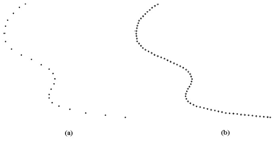
\includegraphics[width=0.2\textwidth]{pre1}
\caption{Digit four (a) Before resampling  (B) After resampling}
 \label{fig:pre1}
 \end{figure}

We noticed that some writers move their hands up while writing the digit which mean more than one stroke in a digit, so we need to group those stokes together then concatenate the strokes into a continuous flow for proper recognition. Linear interpolation simply concatenates the strokes, as shown in Fig.\ref{fig:pre2}.

%We noticed that some writers move their hands up while writing the digit which mean more than one stroke in a digit, so we need to group these stokes together then concatenate the strokes into a continuous flow,as shown in  Fig. .


 \begin{figure}
 \centering
 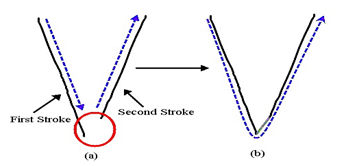
\includegraphics[width=0.2\textwidth]{pre2}
\caption{Linear interpolation concatenates the strokes of digit 7 } \label{fig:pre2}
 \end{figure}

 As shown in Figure \ref{fig:pre2}, the linear interpolation solved the problem of more than one stroke in a digit . Another problem is writing more than one stroke in a digit and changing the direction of the writing flow in the second stroke which results in deforming the digit , as shown in Fig \ref{fig:pre3}.
 \begin{figure}
 \centering
 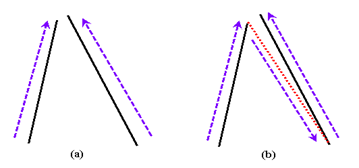
\includegraphics[width=0.25\textwidth]{pre3}
 \caption{ (a) Example of changing direction , (b) direct interpolation deforms the digit.}
  \label{fig:pre3}
  \end{figure}

The previous problem cannot be solved using interpolation directly , the first step to solve this problem is to locate the pen up and pen down location, the end and the start of the second stroke is tested to determine the direction of the stroke. If the user changed the writing direction of the second stroke; the points of the second stroke will be reversed before Interpolating the points,as shown in Fig \ref{fig:pre4}.

 \begin{figure}
 \centering
 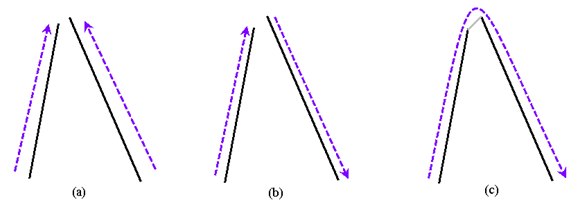
\includegraphics[width=0.25\textwidth]{pre4}
 \caption{(a) Original writing order (b) changing the direction , (c) interpolation }
\label{fig:pre4} \end{figure}
The resampling stage also adjusts the number of $(X,Y)$  points in each digit to a fixed number (80, empirically) for classification purposes.
%Finally , Adjusting the number of  points in each digit to a fixed number (70, empirically) for classification purposes.

 \subsection{Smoothing}
To eliminate the noise, we perform smoothing using 5-point moving average algorithm \cite{Matlab} as shown in Fig \ref{fig:pre55}.

 \begin{figure}
 \centering
 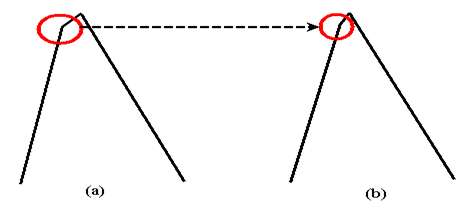
\includegraphics[width=0.25\textwidth]{pre5}
 \caption{Digit 8 (a)	Output from resampling , (b) after smoothing}
\label{fig:pre55}
 \end{figure}


\section{Feature Extraction}
\label{sec:FeatureExtraction}
Feature extraction is the most important factor in achieving a good recognition rate. After studying various feature extraction methods, we selected a mixed feature vector containing a variety of temporal and spatial  features.


\subsection{Temporal Features}
\label{sec:temporal}
The temporal features are features based on the on-line information of the users input stroke. They are computed for each point in the user's pen path. The stroke is defined as  $P(t_i)=(x(t_i),y(t_i))$, $i=1, 2, 3..N$, where  $P(t_i)$ is the  point at instant $t_i$ and  $N$= 80 is the number of points that represent the digit.  The following features are computed:

%\begin{enumerate}[a]
\subsubsection{ F1: Directional Feature}
     The local writing direction at a point $P(t)=(x(t),y(t))$ at instant $(t)$ is described by cosine and sine \cite{Jaeger2001}:
\[
\begin{array}{l}
 \cos (\alpha (t)) = \frac{{\Delta y(t)}}{{\Delta s(t)}} \\
 \sin (\alpha (t)) = \frac{{\Delta x(t)}}{{\Delta s(t)}} \\
 \end{array}
\]
where $\Delta x(t)$ , $\Delta y(t)$ and $\Delta S(t)$ are defined as follows:
\[
\begin{array}{l}
 \Delta x(t) = x(t - 1) - x(t + 1) \\
 \Delta y(t) = y(t - 1) - y(t + 1) \\
 \Delta s(t) = \sqrt {\Delta x^2 (t) + \Delta y^2 (t)}  \\
 \end{array}
\]


 \begin{figure}
	\centering
		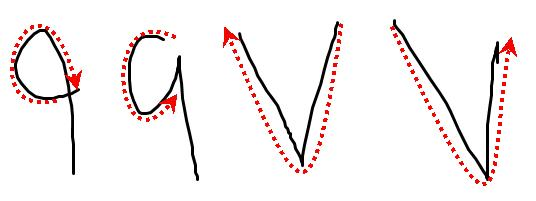
\includegraphics[scale=0.35]{79}
	\caption[ Writing Direction] {Various writing order of digits 7 and 9.}
	\label{fig:direction}
\end{figure}

Our experiments showed that the dependence on temporal features only was insufficient because the order of writing of some Arabic digits is not the same among different writers as shown in Fig. \ref{fig:direction}. Also, some writers tend to over-write some strokes of some digits as shown in Fig. \ref{fig:direction2} and, thus, the system gets confused and gives wrong results. Therefore, spatial features which describe the global shapes of the digits have been used.


  % The first set of features we used was the directional features only. Figure  shows the writing direction of Arabic digit '9' and '7'. It is clear that the writing direction is different and can be used to discriminate different digits. Unfortunately, the test found that some digits written in various directions can't be classified as shown in Fig. The figure shows that when a users change the writing direction more than once (or Over trace a digit), the system get confused and gives wrong results. This means that depending on directional features only is not enough and  thus  we tried to use other features which describe the global digit.% Those features are described in the following section to solve the previous problem.


 \begin{figure}
	\centering
		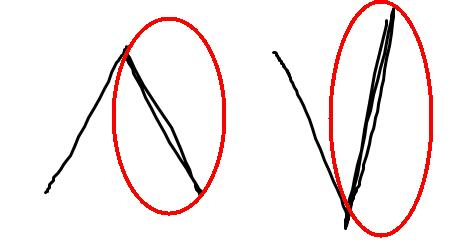
\includegraphics[scale=0.35]{direction2.jpg}
	\caption[ Writing Direction] {The over-tracing in writing a digit.}
	\label{fig:direction2}
\end{figure}



\subsection{Spatial Features}
\label{sec:spatial}

Before extracting the spatial features, the the user's  strokes are converted into a bitmap image. The image is created from the on-line stroke by first connecting the stroke points by straight lines, then the image is resized to a normalized size of $30X30$ . The spatial features used are divided into global shape descriptors  and global concavity features.
\subsubsection{F2:Global Features}

\begin{itemize}
\item The aspect ratio characterizes the height-to-width ratio of the bounding box containing the digit.
\[
    Aspect=\frac{Height}{Width}
\]
where $Height$ and $Width$ are the height and width of image before resizing.


\item The area of the bitmap image $area=Height\times Width$

\end{itemize}

\subsubsection{ F3: Concavity Features}
\label{sec:F3}
The following concavity features are computed on the bitmap image $30X30$  . The features describe the visual appearance of the digits and they represent  a subset of several spatial features used for off-line Arabic digits recognition in \cite{Abdelazeem2009}. Figure \ref{fig:features} shows the concavity features.
\begin{enumerate}
    \item 'W2':  Number of white pixels between the black pixels at the top of the digit, the black pixels at the left of the digit, the black pixels at the bottom of the digit, and the right corner of the bounding box. This feature distinguishes digit 2.
     \item    'W3':  Number of white pixels surrounded by black pixels to their right and left and by the top corner of the bounding box from above. This feature distinguishes digit 3.
   \item 'W4' : Number of white pixels surrounded by black pixels from above and below and having the left corner of the bounding box to their left. This feature distinguishes digit 4.
    \item 'W5': Number of white pixels surrounded by black pixels in all directions. This feature distinguishes digit 5.
     \item  'W6' : Number of white pixels surrounded by black pixels from above and right and by the left and bottom corners of the bounding box. This feature distinguishes digit 6.
      \item  'W7': The last row from the bottom that has 'W3' pixels is considered the depth of the 'W3' pixels. This feature differentiates between digits 3 and 7.% The last row from the bottom that has 'W3' pixels is considered the depth of the 'W3' pixels. differentiate between digit 3 and 7.
  \item  'W8':  Number of white pixels surrounded by black pixels to their right and left and by the bot tom corner of the bounding box from below. This feature distinguishes digit 8.
  \item 'W9':  Number of white pixels surrounded by black pixels in all directions in the upper left half of the bounding box. This feature distinguishes digit 9.
   \item 'B69': The average height of the black pixels in the left half of the bounding box (That is, the distance between the first black pixel in one column and the last black pixel in the same colunm averaged over all the columns of the left half of the bounding box). This feature differentiates between digits 6 and 9.
\end{enumerate}

\begin{figure}[h]
\centering
 \subfigure['W2']{\label{fig:fig3}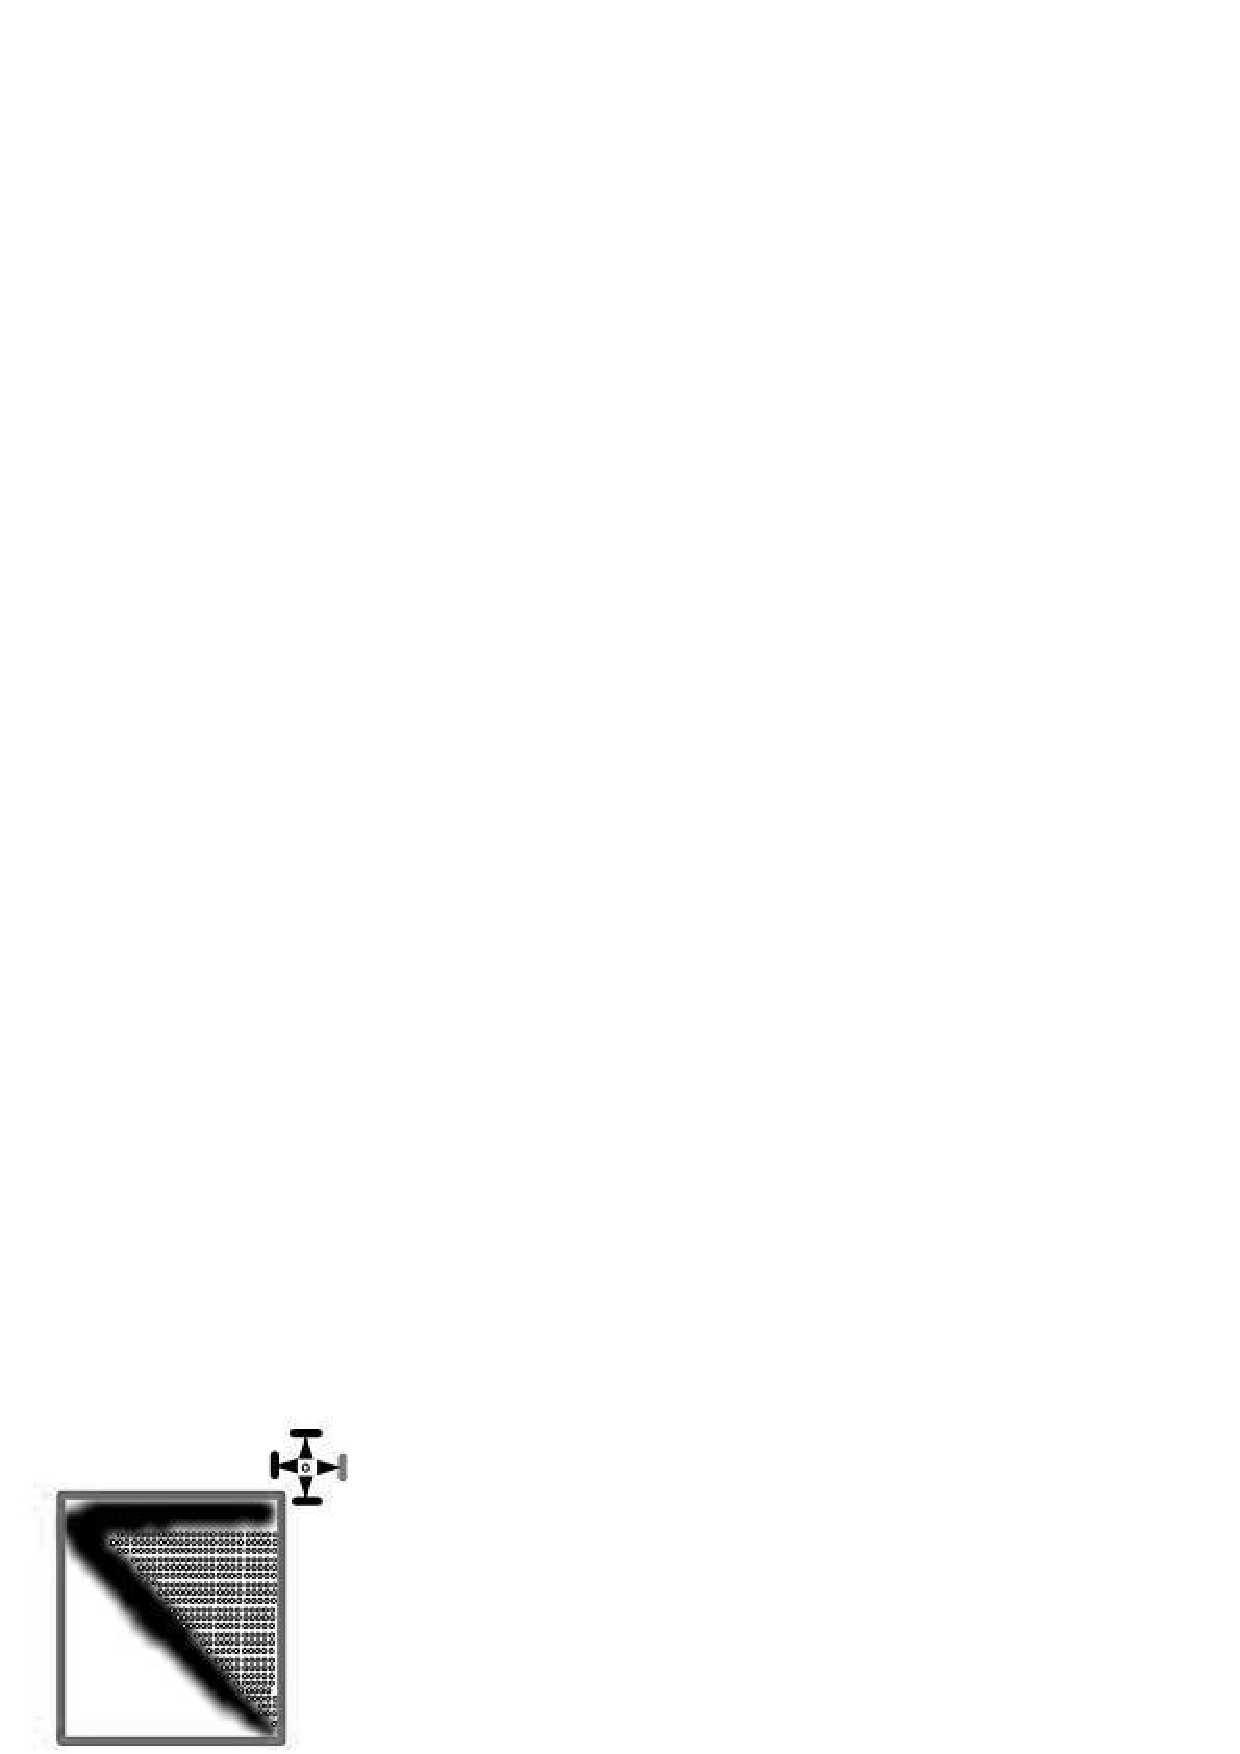
\includegraphics[width=0.08\textwidth]{figures/fig3.jpg}}
 \subfigure['W3']{\label{fig:fig4} 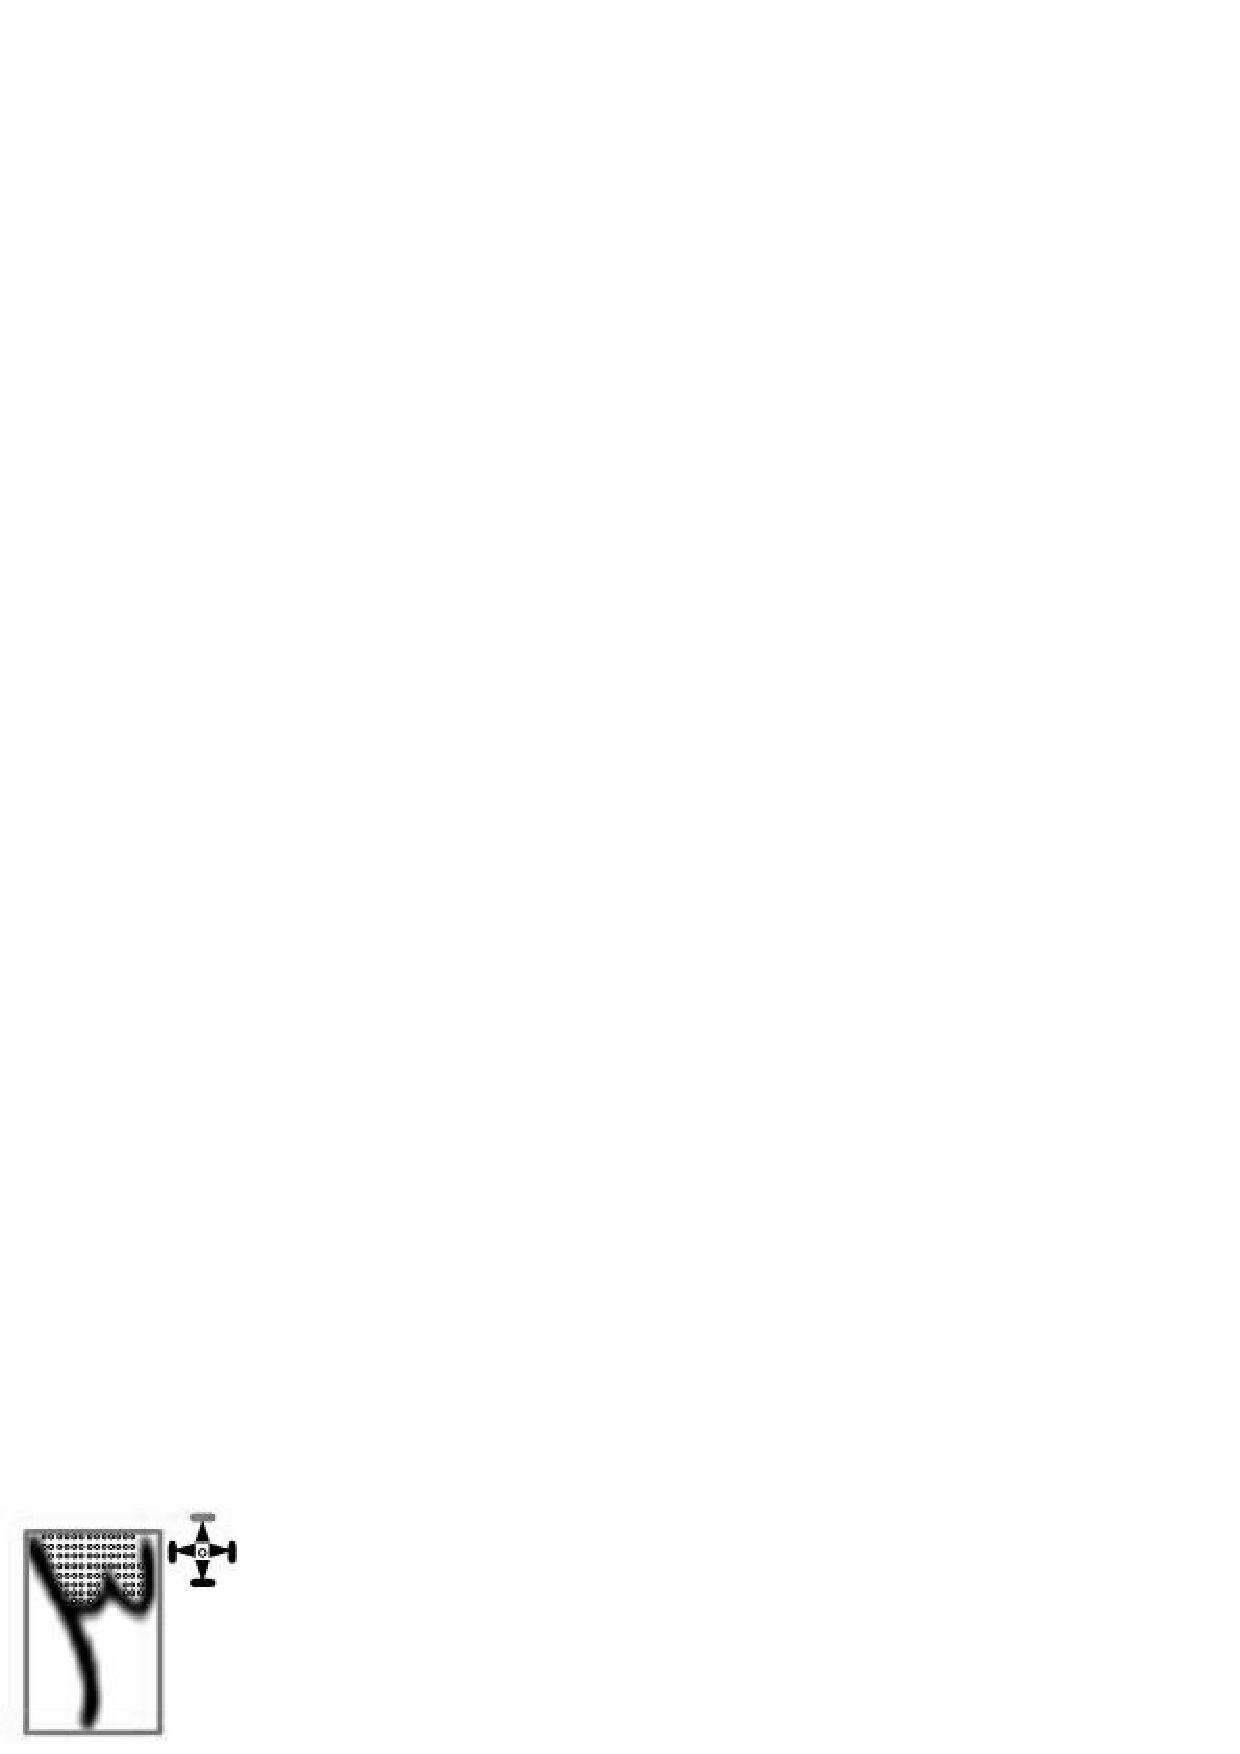
\includegraphics[width=0.08\textwidth]{figures/fig4.jpg}}
\subfigure['W4'.]{\label{fig:fig5}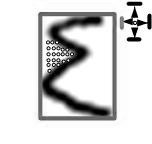
\includegraphics[width=0.08\textwidth]{figures/fig5.jpg}}
  \subfigure['W5']{\label{fig:fig6}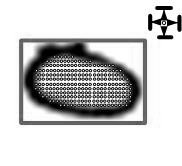
\includegraphics[width=0.08\textwidth]{figures/fig6.jpg}}
 \subfigure['W6]{\label{fig:fig7}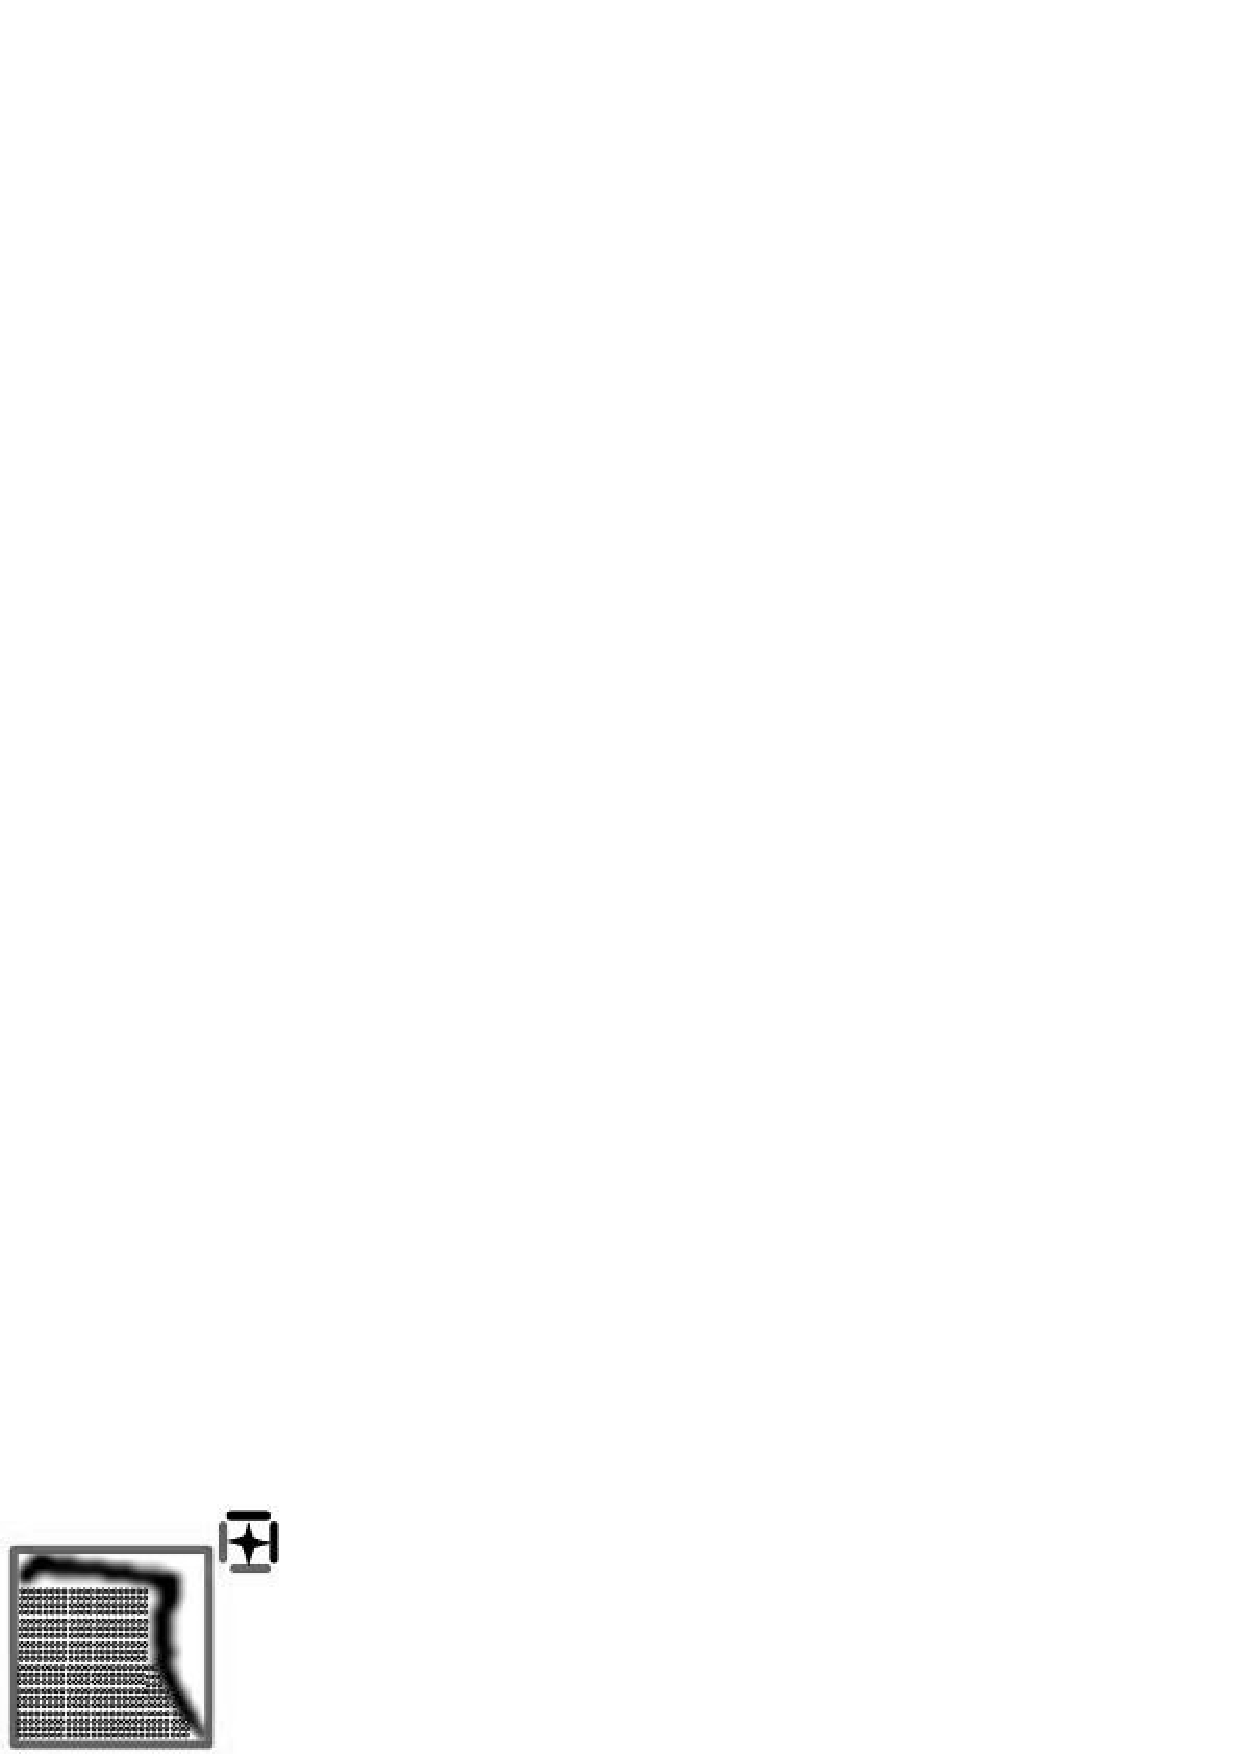
\includegraphics[width=0.08\textwidth]{figures/fig7.jpg}}
   \subfigure['W7']{\label{fig:fig9b}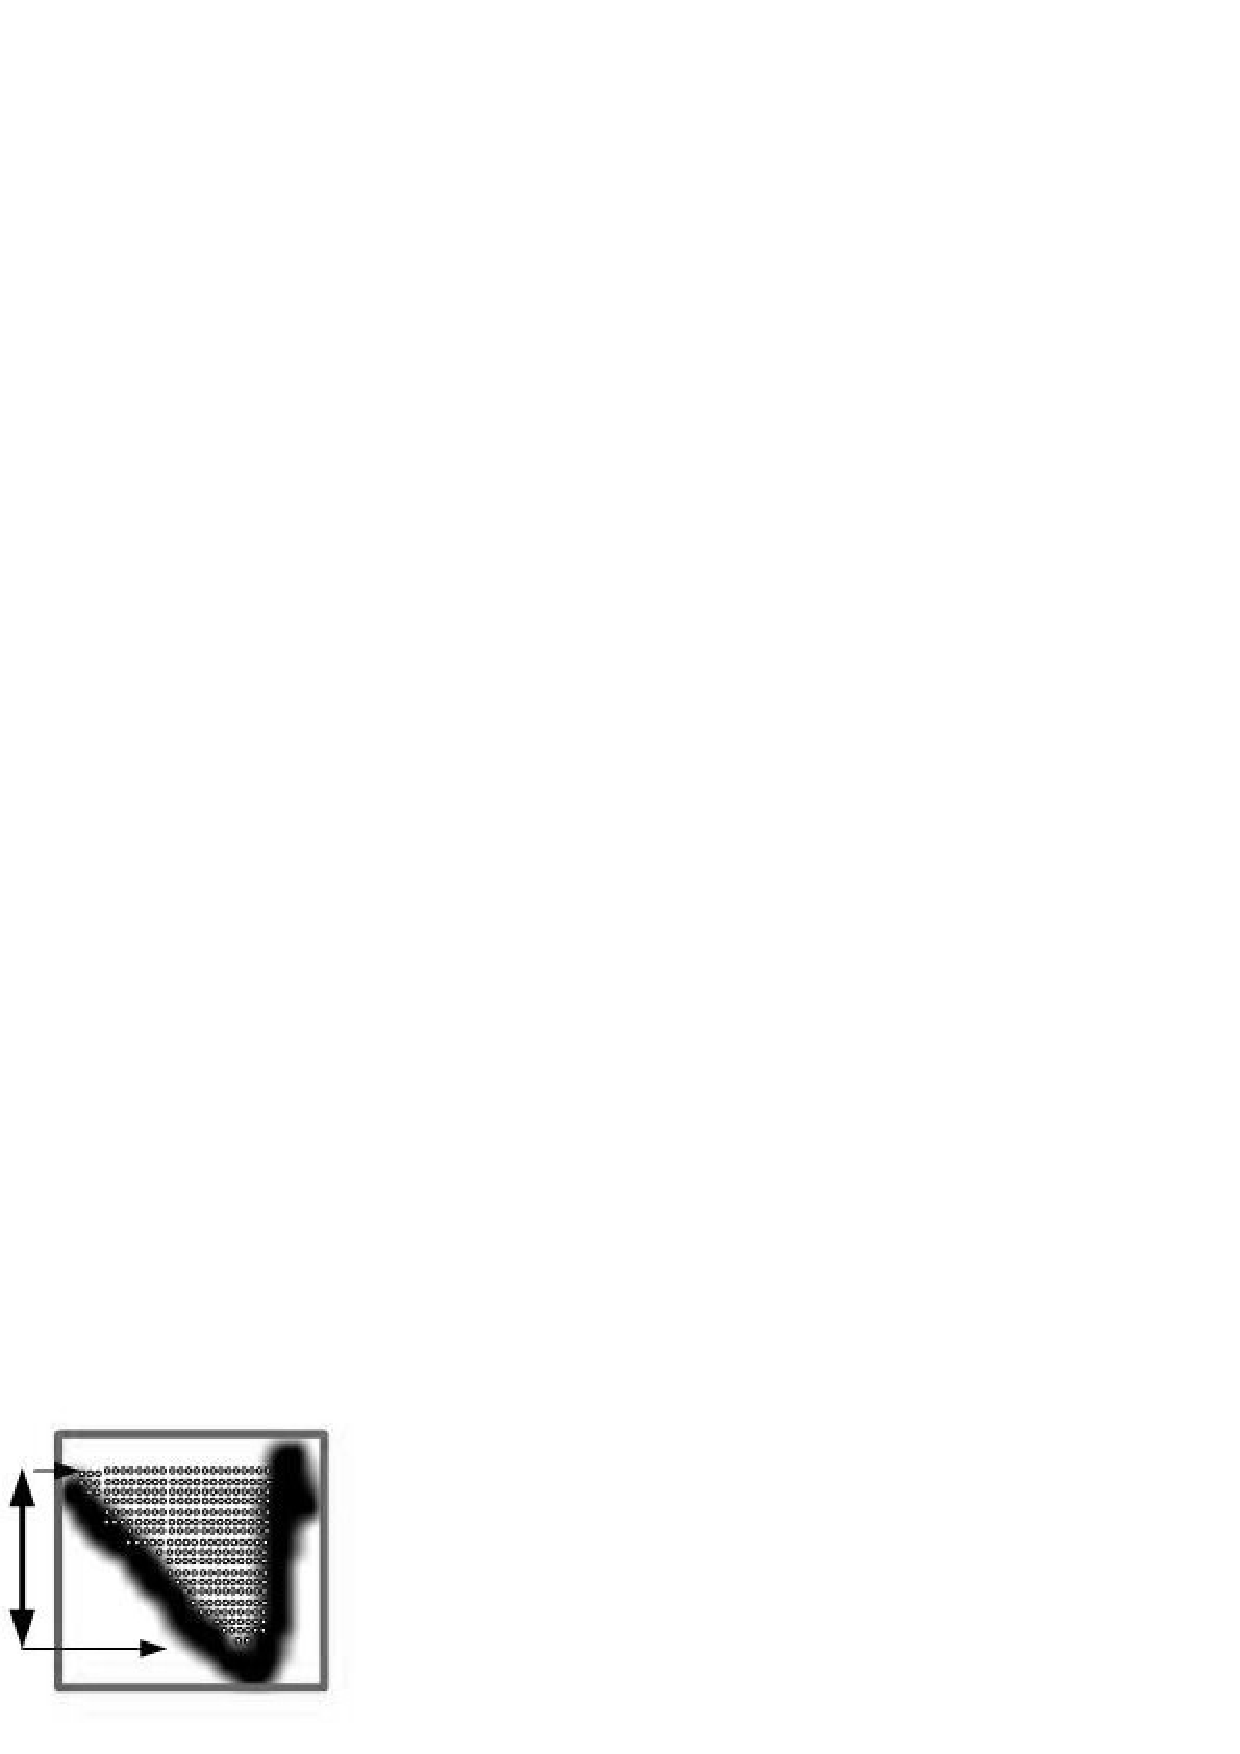
\includegraphics[width=0.08\textwidth]{figures/fig9b.jpg}}
    \subfigure['W8]{\label{fig:fig9}\includegraphics[width=0.08\textwidth]{figures/fig10.jpg}}
     \subfigure['W9']{\label{fig:fig11b}\includegraphics[width=0.1\textwidth]{figures/fig11b.jpg}}
\subfigure['B69']{\label{fig:fig11b}\includegraphics[width=0.1\textwidth]{figures/fig12b.jpg}}
 % \subfigure[Feature 'White\_3'.]{\label{fig:fig8}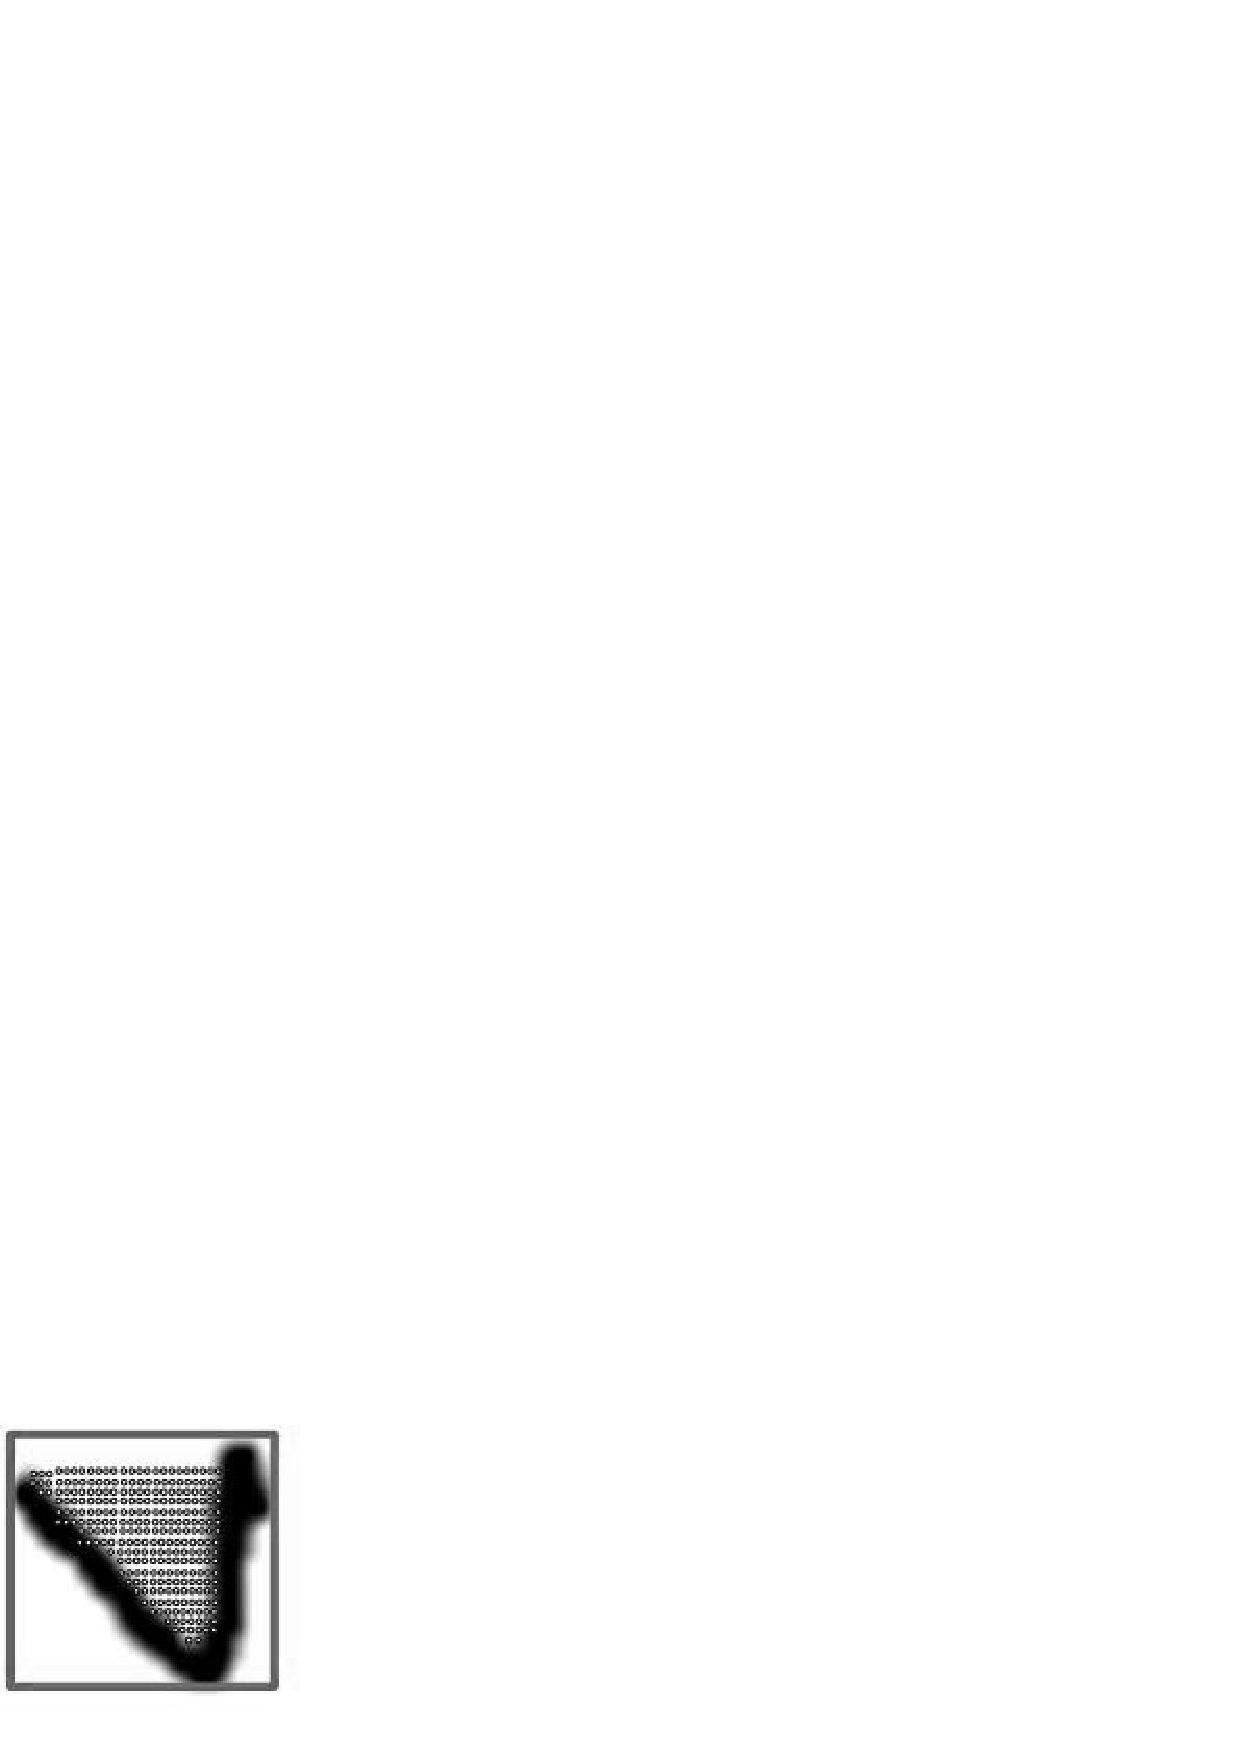
\includegraphics[width=0.13\textwidth]{figures/fig8.jpg}}
 \caption{Examples of the Spatial Features}
 \label{fig:features}
\end{figure}


\subsection{Digit Zero Problem}
\label{sec:ZeroProblem}



The Arabic Digit zero '0' is very difficult to recognize because it has no specific way to write it, as it is only like a decimal point. Figure \ref{fig:zerosize} shows different samples of the Arabic Digit '0'. The figure clearly shows that the digit has no specific way of writing  and it usually confuses with other digits especially Arabic digits '1' and '5'. The most discriminating feature for the digit '0' over the other digits is its size and number of points used to write it. Figure \ref{fig:zeroVersusOther} shows the average size of Digit '0' versus other Arabic digits. Since digit '0' is written in a small area and random direction, it is better be recognized separately




 \begin{figure}
	\centering
		
\includegraphics[scale=0.35]{Zero0}
	\caption[Arabic '0' Digits ] {Different samples of the Arabic Digit '0'}
	\label{fig:zerosize}
\end{figure}


 \begin{figure}
	\centering
		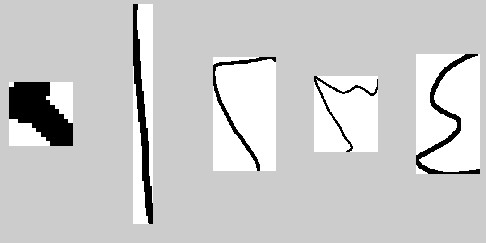
\includegraphics[scale=0.2]{Zero1}
	\caption[Arabic '0' Digits Versus Other digits] {The difference in size between digits '0' and other digits..}
	\label{fig:zeroVersusOther}
\end{figure}

%Figure \ref{fig:flowChart} shows a block diagram of the recognition system. The system is divided into three main blocks; Pre processing, Zero recognizer and Final Classifier.  In Pre Processing the stroke are re-sampled and smoothed. The second stage is recognizing the zero digit using a SVM classifier the output of this stage is either labeling the digit as a zero or continuing to the next stage. The final stage is on-line and offline OVO classifier.
 Consequently,  our final system is composed of two classification stages, the first stage recognizes the digit '0' and the second stage recognizes the rest of the digits. Figure \ref{fig:flowChart} shows a block diagram of our recognition system. The system is divided into three main blocks; Preprocessing, digit '0' recognizer, and a final Classifier. The first classification stage output is either labeling the digit as a zero or continuing to the next stage. The final stage discriminates between Arabic digits from 1 to 9.

 \begin{figure}
	\centering
		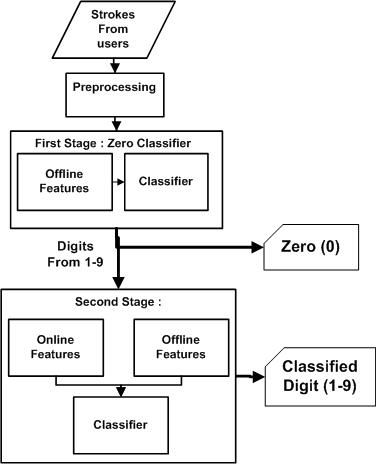
\includegraphics[scale=0.45]{Block}
	\caption[System Block Diagram] {The system block diagram}
	\label{fig:flowChart}
\end{figure}


\subsubsection{Digit Zero Classifier }
\label{sec:DigitZeroClassifier}
%As mentioned above, it is clear that the Arabic Digit '0' will need offline features to be distinguishible from others digits. The main feature that differentiates between 0 and other digits is the size, number of points and aspect ratio. Our experiments showed they were not enough to get the high accuracy required in the first stage. Therefore we tried various other offline features to detect the Arabic Digit '0'. The number of transitions from white pixels to black pixel and vice-versa in a specific direction (see Fig \ref{fig:featTrans}) proved to be very effective for this purpose. To reduce the dimensionality of the feature vector we chose to take only 3 transitions in every direction: vertical, horizontal, left diagonal, and right diagonal.


As mentioned above, it is clear that the Arabic Digit '0' will need offline features to be distinguishible from others digits. The main feature that differentiates between 0 and other digits is the size, number of points and aspect ratio. Our experiments showed they were not enough to get the high accuracy required in the first stage. Therefore we tried various other offline features to detect the Arabic Digit '0'. The number of transitions from white pixels to black pixel and vice-versa in a specific direction (see Fig. \ref{fig:featTrans} ) proved to be very effective for this purpose. To reduce the dimensionality of the feature vector we chose to take only 3 transitions in every direction: vertical, horizontal, left diagonal, and right diagonal.

Figure \ref{fig:featTrans} shows that Arabic digit '0' can be distinguished from other digits as it has a single transition in all direction in contrast to other digits. For example, digit  '4' has a high number of  vertical transitions and digit '8' has a high number of transitions in the horizontal direction.


%As mentioned above it was clear that the Arabic Digit '0' will need offline feature to be discriminable from others digits. The main feature that differentiates between 0 and other digits is the size, number of points and aspect ratio. Unfortunately, they are not enough to get high accuracy required in the first stage. Therefore we tried various offline features to detect the Arabic Digit '0'. Finally, we choose to computes the number of transitions from white pixels to black pixel and vice-versa in a specific direction

   %Figure \ref{fig:featTrans} shows that Arabic digit '0' can be distinguished from other digits as it has a single transition in all direction. In contrast to other digits as for example, '4' has high number of transition vertical transition and digit '7' has high number of transition in horizontal direction.
    %set of feature %Trying to get the best result we tried various feature sets to finally choose the best feature set. %The following list describes the three different features set that were used to test the Zero Classifier. %We then compared three set of feature to achieve the better results. The first set of features is the same as offline features in the second stages.

 \begin{figure}
	\centering
		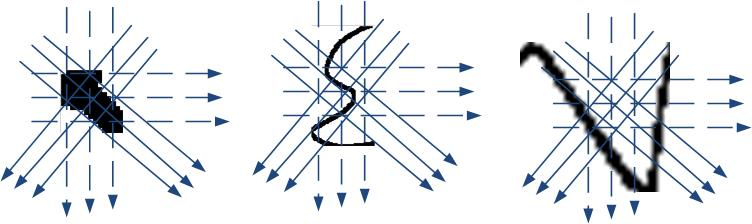
\includegraphics[scale=0.3]{Trans2}
	\caption[Transition features] {The direction of transition features in digit '0' , '4' and '8' }
	\label{fig:featTrans}
\end{figure}
% \begin{itemize}
%   \item Connectivity-FS: Some of the features mentioned in section \ref{sec:F3}. The feature vector consist of only ('White 2', 'White 3', 'White 4', 'White 5', 'White 6','White 8' 'White 9').
%   \item Transitions-FS : The number of transition from black to white and vise vera. To reduce the dimensionality of the feature vector we choose to take only 3 in every direction of vertical, horizontal, left diagonal and right diagonal.
%
%   \item Projection-FS : The projections of the bitmap image of the digit.  To reduce the dimensionality of the feature vector we choose to take only 3 in every direction of vertical, horizontal , left diagonal and right diagonal.
%
% \end{itemize}
%
% As mentioned, the area, aspect ratio and number of points in the stroke are main features for the Arabic digit Zero. These three main features were added to each of the previous feature set and a test was conducted to choose the best feature set. The comparison for each of the feature sets are explained in the results section.
%

 %In the Zero classifier we started by testing feature set F3.  Then tried a second set of features;   the final feature. Also we choose to take only 3 columns in every direction to extract these features.

%Zero features :MAHA


\section {Results}
\label{sec:Results}


The system is composed of two stages (see Fig \ref{fig:flowChart} ). The first stage is the Digit Zero Classifier and the second stage is used to classify digit from (1 to 9). Since the first stage focuses only on the  digit '0', we used single linear SVM classifier. However, we needed a multi class classifier for the second stage. The nonlinear SVM is originally designed for 2-class problems. Extending it to multi-class can be done using the One Versus One (OVO) or the One Versus All (OVA) schemes. We used the OVO scheme to classify 9 digits which means we have 36 linear classifiers in the second classification stage.

The input feature vector for the first stage consists of 15 features divided into 12 transition features and three global feature. (see Section \ref{sec:DigitZeroClassifier}). The second stage uses a multi-class nonlinear SVM classifier with input feature vector of length 166. The 166-elements feature vector is a concatenation of the following features: F1 (156 elements), F2 (2 elements), F3 (9 elements) as explained in Sections   \ref{sec:temporal} and  \ref{sec:spatial}.

The collected AOD dataset is divided into 80\% of the writers as training set and 20\% of the writers as test set. All the result given here are computed on the test set. The accurcay is defined as the nubmer of correctly classified digits divided by the total number of digits in the test set. Table \ref{tab:ResultsStage1} shows the accuracy of the different stages of the system. The results show that the first stage achieved accuracy of 99.69\% and the second stage achieved an accuracy of 98.89\% on digits from 1 to 9 only. Table \ref{tab:ResultsStage1} shows that the overall accuracy of the system is 98.73\%. Figure \ref{fig:conff} shows a sample of some of the confused digits.



  %   The system is composed of two stages (see Fig \ref{fig:flowChart} ).  The first stage is a Digit Zero Classifier and the second stage is used to classify digit from (1  to 9). Since the first stage focus only on the zero digits we used single linear SVM classifier. However, we needed a multi class classifier for the second stage. The nonlinear SVM is originally designed for 2-class problem. Extending it to multi-class can be done using the One Versus One (OVO) or the One Versus All (OVA) schemes. We used the OVO scheme to classify 9 digits which means we have 36 linear classifiers.

   %  The input feature vector for the first stage consist of 15 features divided into 12 transition features and three global feature. (see section \ref{sec:DigitZeroClassifier}). The second stage uses a multi-class nonlinear SVM classifier with input feature vector of length 166 for second stage. The (166 )-element feature vector is a concatenation of the following feature: F1 (156 elements), F2 (1 element), F3 (9 elements).

    % The collected AOD dataset is divided into 80\% of the writers as trainset and 20\% of the writers as testset. All the result shown are computed on the testset. The accurcay is defined as the nubmer of correctly classified digits divided by the total number of digits in the testset.  Table \ref{tab:ResultsStage1} shows the accuracy of the different stages of the system. The results shows that the first stage achieved accuracy of 99.6899\%  and the second stage which consist of OVO non linear SVM classifer achieved an accuracy of  98.89\%  on digits from 1 to 9 only. Table \ref{tab:ResultsStage1} shows that the overall accuracy of the  system is 98.73\%.  Figure \ref{fig:conff} shows a sample of some of the confused digits.  % first stage. The table shows the result of each of the feature set discribed in section \ref{sec:ZeroProblem}. The results shows that the Connectivity-FS and  Transitions-FS features set have the best recognition rate.

%      Table \ref{tab:Results}  shows the accuracy of the whole system. The accuracies of each features for each stage of the system and the accuracy of whole system are presented. The table clearly shows that online features achieve better accuracy then offline feature and that combining them improves the accuracy.

\begin{table}[h]
\begin{center}
\caption[First Stage result table]{ Results of different stages }
%\scalebox{0.8}{
 \begin{tabular}{|c|c|}
 \hline
Stage &   Accuracy   \\ \hline
	Stage 1  &  99.69\%  \\ \hline
    Stage 2  & 98.89\% \\ \hline
	Overall System  &  98.73\%  \\   \hline

\end{tabular}
\label{tab:ResultsStage1}
\end{center}
\end{table}

 \begin{figure}
	\centering
		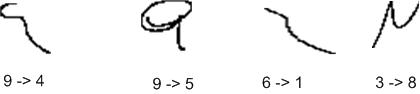
\includegraphics[scale=0.4]{conf2.jpg}
	\caption[ A sample of the misclassified digits by the proposed system.]{}
	\label{fig:conff}

\end{figure}
% \begin{table}[h]
% \begin{center}
% \caption[First Stage result table]{ Results of different stages }
% %\scalebox{0.8}{{
%  \begin{tabular}{|p{1in}|c|c|c|c|c|c|c|c|c|c|c|}
%   \hline
%  Actual/Perdicted & 1&2&3&4&5&6&7&8&9 \\   \hline
% 0&0	&0&	0&	0 &	3&	1&	0&	0&	0 \\   \hline
% 1&2&	0 &	2 &	3&	1&	0&	0&	0&	1	 \\   \hline
% 2&0&	9 &	0 &	0&	0&	0&	0&	0&	3	 \\   \hline
% 3&0&	0 &	0 &	0&	0&	0&	0&	0&	1	 \\   \hline
% 4&0&	0 &	10 &	1&	0&	0&	0&	0&	2	 \\   \hline
% 5&0&	0 &	0 &	0&	0&	0&	0&	1&	2	 \\   \hline
% 6&14&	0 &	1 &	0&	0&	1&	0&	0&	0	 \\   \hline
% 7&0&	0 &	0 &	0&	0&	1&	0&	0&	0	\\   \hline
% 8&0&	4 &	0 &	1&	1&	3&	0&	0&	0	\\   \hline
% 9&1&	0 &	0 &	0&	1&	0&	0&	0&	0	\\   \hline
% \end{tabular}
% \label{tab:ResultsStage1}
% \end{center}
% \end{table}

% \begin{table}[h]
% \begin{center}
% \caption[Results]{Table compares between Results of different feature sets}
% %\scalebox{0.8}{
%  \begin{tabular}{|c|c|c|c|}
%  \hline
%  	Features	& Accuracy \\ \hline
%     Offline	 &    97.48\%\\   \hline
%  	Online	& 98.62 \\ \hline
%  	Online and Offline & 98.73\%  \\ \hline
%
% \end{tabular}
% \label{tab:Results}
% \end{center}
% \end{table}


\subsection{Comparison with commercial products}


%Vision Objects: They have built cursive Arabic handwriting recognition system for ICDAR 2009 Online Arabic Handwriting Recognition Competition \cite{ICDAR2009} based on MyScript handwriting recognition technology. They have designed the recognizer according to two different criteria. The first system (VisionObjects-1) provides the best accuracy whereas the second system (VisionObjects-2) is faster in exchange for a somewhat lower accuracy. We compared our system with MyScript Studio Notes Edition and we found that:
%The recognition rate for digits in MyScript system is lower than our system because the digits are confused with isolated Arabic characters as shown in Fig\ref{fig:scriptresult}. Figure \ref{fig:scriptresult} shows that MyScript confuse Arabic digit '1' with Arabic letter Alef  and   Arabic digit '4' with Arabic letter Ein.


Vision Objects has built a cursive Arabic handwriting recognition system for the ICDAR 2009 On-line Arabic Handwriting Recognition Competition\cite{ICDAR2009} called MyScript Studio Notes Edition \cite{MyScript}. MyScript Studio Notes Edition attained the first place in the ICDAR 2009 competition. We choose to compare our system to MyScript Studio Notes Edition as one of the best commercial handwriting systems available today. Ten of our test set writers have been asked to write Arabic digits on My Script Notes Edition as shown in Fig.\ref{fig:figpaper}.


%Vision Objects has built a cursive Arabic handwriting recognition system for ICDAR 2009 Online Arabic Handwriting Recognition Competition \cite{ICDAR2009} called MyScript Studio Notes Edition\cite{MyScript}. MyScript Studio Notes Edition attained the first place in ICDAR 2009 competition. We choose to compare our system to MyScript Studio Notes Edition as on of the best  commercial handwriting systems. Ten of our test set writers have been asked to write Arabic digits on My Script Notes Edition as shown in  Fig\ref{fig:figpaper}.


%MyScript handwriting recognition technology.
 %They have designed the recognizer according to two different criteria.  The recognition rate for those test  digits on MyScript system is much lower than our system's recognition rate  for the same digits  as shown in Table \ref{tab:ResultsMyScript}.


 The results of My Script recognition are shown in Fig. \ref{fig:scriptresult}. It is clear from the figure that My Script confuses many Arabic digits with other Arabic characters or Latin digits because of the similarity in visual appearance with those characters. For example, Arabic digit '4' is confused with Arabic character 
\includegraphics[scale=0.2]{ean.jpg} and Arabic digit '5' is confused with Arabic character  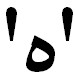
\includegraphics[scale=0.2]{haa.jpg}. Also, Arabic digit '0' could not be recognized at all by My Script. This poor performance takes place because My Script recognizes both Arabic Characters and digits in one system. Our proposed system is dedicated to the recognition of Arabic digits only and, thus, produces superior results as reported in Table \ref{tab:ResultsMyScript}.


  %The results of My Script recognition are shown in Fig.  \ref{fig:scriptresult}. It is clear from the figure that My Script confuses many Arabic digits with other Arabic characters or Latin digits because of the similarity in visual appearance. For example, Arabic digit '4' is confused with Arabic character ' ع' and Arabic digit '5' is confused with Arabic character 'ه'. Also, Arabic digit '0' could not be recognized at all by My Script. This poor performance takes place because My Script recognizes both Arabic Characters and digits in one system. Our proposed system is dedicated to recognition of Arabic digits only and, thus, produces superior results.

\begin{figure}[h]
\centering

  \subfigure{\label{fig:figpaper}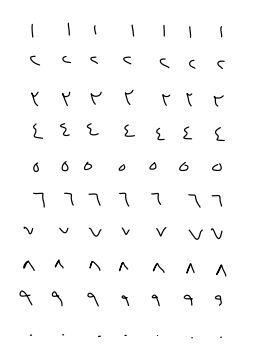
\includegraphics[width=0.17\textwidth]{page.jpg}}
  %\subfigure[Feature 'White\_3'.]{\label{fig:fig8}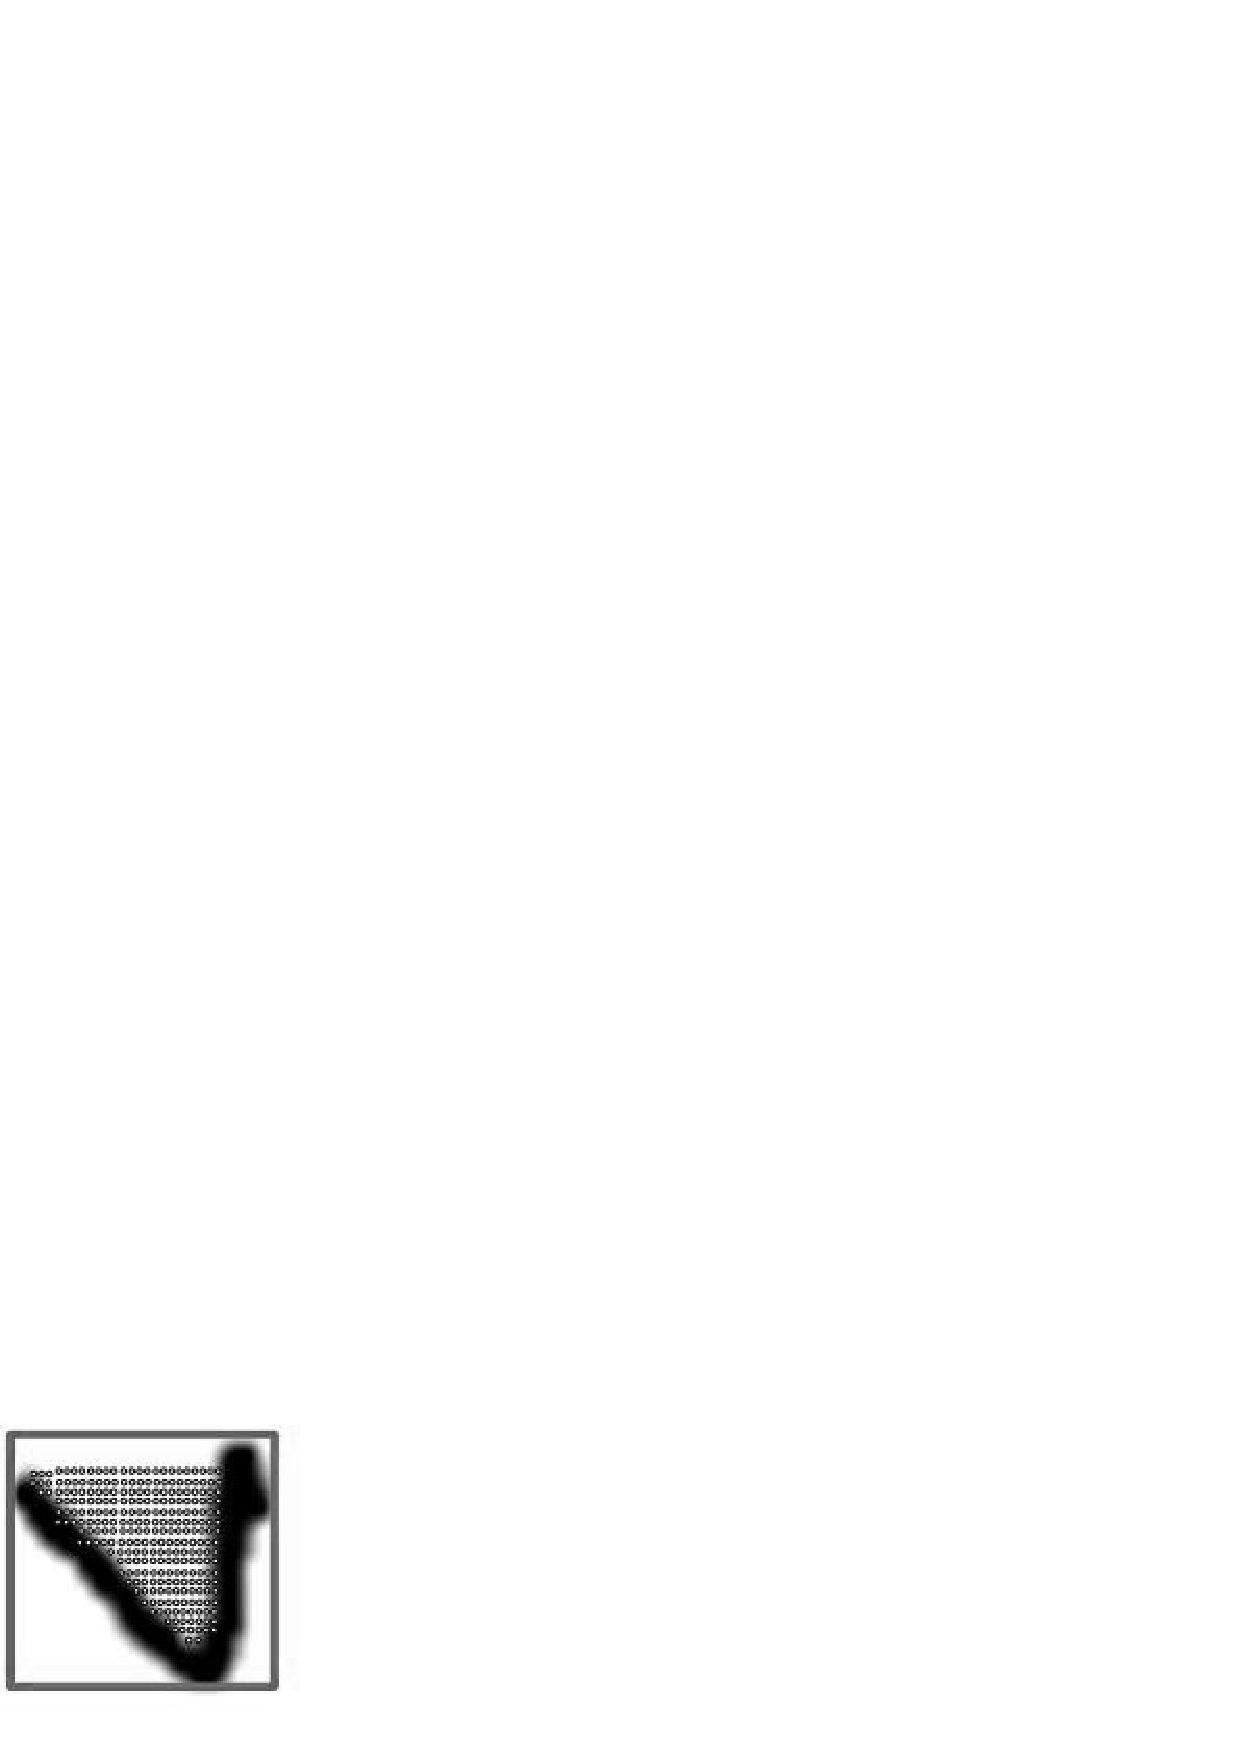
\includegraphics[width=0.15\textwidth]{figures/fig8.jpg}}

    \subfigure{\label{fig:scriptresult}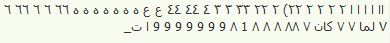
\includegraphics[width=0.35\textwidth]{res.jpg}}
 \caption{(a)Test digits (b) My Script results}
\end{figure}


%The results for MyScript Studio Notes Edition are shown in Table \ref{tab:ResultsMyScript} which shows the result of 10 writers of the dataset compared to result from our system. The result shows that MyScript achieve lower result than our system because our systems focus on the specific digit problem.
\begin{table}[h]
\begin{center}
\caption[Results]{Comparison between the results of the proposed system and those of My Script for the input test digits.}
%\scalebox{0.8}{
 \begin{tabular}{|c|c|c|c|}
 \hline


System   & Accuracy \\ \hline
Our System  & 99.64\% \\ \hline
MyScript & 70.69\%  \\ \hline

\end{tabular}
\label{tab:ResultsMyScript}
\end{center}
\end{table}


\section{Conclusion}
\label{sec:Conclusion}
  In this paper we presented a system that uses both temporal and spatial information to recognize on-line Arabic digits. A new on-line Arabic digit dataset was collected to test the performance of the proposed system. The dataset consists of 30,000 samples collected from 300 different writers. The proposed system is divided into two main classification stages, the first stage is to recognize the Arabic digit zero and the second stage is to recognize the remaining digits. The overall recognition rate achieved is 98.73\%. The paper also presented a comparison with a commercial system and the results show that the proposed system is more efficient as it focuses on the digits recognition problem only.


\bibliographystyle{IEEEtran}
\bibliography{Library}
% that's all folks
\end{document}
